\documentclass[12pt]{article}
\usepackage{fancyhdr}
\usepackage[colorlinks=true,
			linkcolor=blue,
			citecolor=blue,
			urlcolor=blue,
			pdfborder={0 0 0}]{hyperref}
\usepackage{graphicx}
\graphicspath{{./results/}{./}}
\usepackage{amsmath}
\usepackage{amssymb}
\usepackage{float}
\usepackage{parskip}
\usepackage{caption}
\usepackage{subcaption}
\usepackage[top=1in,bottom=1.2in,left=1in,right=1in]{geometry}

\parskip=\baselineskip
\parindent=0pt

\pagestyle{fancy}
\fancyhf{}
\fancyfoot[R]{\raisebox{5pt}{\thepage}}
\renewcommand{\headrulewidth}{0pt}
\renewcommand{\footrulewidth}{0pt}

\fancypagestyle{plain}{%
  \fancyhf{}
  \fancyfoot[R]{\raisebox{5pt}{\thepage}}
}

\begin{document}

\pagenumbering{gobble}

\begin{titlepage}
	\centering
	\vspace*{0.01cm}

	
\includegraphics[width=0.4\textwidth]{iisermlogo.png}\\

	\vspace{1.8cm}

	{\Huge\bfseries Synchronization in Complex Networks

	\vspace{1.1cm}

	\Large Course: Modelling Complex Systems\\
	\Large Assignment: Phase Synchronization on Watts-Strogatz Networks\\

	\vspace{\baselineskip}
	Submitted by\\
	\Large Avneesh Singh (MS23249)

	\vspace{1.8cm}

	\large April 23, 2026

	\vfill
}
\end{titlepage}

\thispagestyle{empty}
\newpage

\pagenumbering{arabic}

%-----------------------------------
\section{Question}

Simulate a system of $N$ coupled phase oscillators given by

\begin{equation}
\dot{\theta}_i = \omega_i + K \sum_{j=1}^{N} A_{ij} \sin(\theta_j - \theta_i), \qquad i = 1,\dots,N.
\label{eq:kuramoto_network}
\end{equation}

The local frequencies $\omega_i$ are drawn from a Gaussian distribution centered at zero with unit variance. The coupling matrix $A_{ij}$ is the adjacency matrix of the network.

Investigate synchronization phenomena on Watts-Strogatz small-world networks. The base lattice is a ring with mean degree $k=6$, so each node is connected to three neighbors on either side.

The task is focused only on synchronization properties, including global coherence, local correlations, phase and frequency locking, spectral signatures, and topology dependent synchronization speed.

%-----------------------------------
\section{Introduction}

Networks are a natural language for many interacting systems. In a network, each node is an individual unit and each edge represents an interaction. In physics and applied systems, this framework helps us connect local interactions to global collective behavior.

Coupled oscillators are one of the simplest and most useful examples of this idea. Each oscillator has its own preferred frequency, but interaction with connected neighbors can pull phases together. When this balance favors coupling, synchronization appears.

Synchronization is important in many real systems such as neural activity, power-grid phase coordination, rhythmic biological processes, and coordinated chemical oscillations. This report studies how synchronization changes with coupling strength and with network topology.

%-----------------------------------
\section{Model Description}

The dynamical model is given by Eq. \eqref{eq:kuramoto_network}. Each term has a direct physical meaning:

\begin{itemize}
	\item $\theta_i$: instantaneous phase of oscillator $i$.
	\item $\omega_i$: intrinsic frequency of oscillator $i$, sampled from $\mathcal{N}(0,1)$.
	\item $K$: global coupling strength that controls interaction intensity.
	\item $A_{ij}$: network adjacency matrix; $A_{ij}=1$ if $i$ and $j$ are connected, and $0$ otherwise.
\end{itemize}

If $K$ is very small, oscillators mostly follow their own frequencies, so phases drift apart. As $K$ increases, interaction terms can overcome this disorder and drive collective phase alignment.

The connectivity is chosen using the Watts-Strogatz construction. It starts from a regular ring and rewires edges with probability $p$. This gives three key regimes used here:

\begin{itemize}
	\item $p=0$: regular lattice,
	\item $p\approx 0.1$: small-world network,
	\item $p=1$: random network.
\end{itemize}

This interpolation is central to synchronization studies because short path lengths and clustering both influence how quickly phase information spreads.

%-----------------------------------
\section{Methodology}

The simulation setup follows the assignment statement and lecture-note conventions.

\subsection{Network generation}
For each run, an undirected Watts-Strogatz network is generated with $N=100$ and mean degree $k=6$. We vary the rewiring probability $p$ depending on the experiment.

\subsection{Initial conditions}
Initial phases are sampled uniformly in $[0,2\pi]$ and natural frequencies are sampled from a standard Gaussian distribution.

\subsection{Time integration}
The coupled ODE system is integrated using fourth-order Runge-Kutta (RK4) with a fixed time step $\Delta t=0.05$. The simulation horizon is chosen long enough to reach steady behavior for most parameter values.

\subsection{Measured observables}
The main synchronization quantities are:

\begin{itemize}
	\item Global order parameter
	\begin{equation}
	r(t) = \left|\frac{1}{N}\sum_{j=1}^{N} e^{i\theta_j(t)}\right|.
	\end{equation}
	\item Time to synchronization, defined from a threshold crossing $r(t)>0.9$.
	\item Pairwise phase correlation $C_{ij}=\cos(\theta_i-\theta_j)$.
	\item Effective frequencies $\Omega_i$ from long-time phase growth.
	\item Power spectral density from oscillator time series.
\end{itemize}

%-----------------------------------
\section{Results and Analysis}

\subsection{Order parameter versus time}

\begin{figure}[H]
\centering
\includegraphics[width=0.8\textwidth]{r_vs_time_lowK.png}
\caption{Time evolution of the global order parameter for low coupling in the small-world network.}
\label{fig:rtime_low}
\end{figure}

Figure \ref{fig:rtime_low} shows weak coherence at low $K$. The order parameter stays small with fluctuations, which means intrinsic frequency disorder dominates interaction.

\begin{figure}[H]
\centering
\includegraphics[width=0.8\textwidth]{r_vs_time_highK.png}
\caption{Time evolution of the global order parameter for strong coupling in the small-world network.}
\label{fig:rtime_high}
\end{figure}

In Figure \ref{fig:rtime_high}, $r(t)$ quickly rises toward one. This is the expected synchronized state where coupling suppresses relative phase drift.

\subsection{Phase evolution in time}

\begin{figure}[H]
\centering
\includegraphics[width=0.8\textwidth]{phase_heatmap_highK.png}
\caption{Heatmap of oscillator phases across time in the synchronized regime.}
\label{fig:heatmap_phase}
\end{figure}

The heatmap reveals increasing alignment across oscillators as time progresses. Uniform color bands indicate that phase differences become small.

\begin{figure}[H]
\centering
\includegraphics[width=0.8\textwidth]{phase_raster_highK.png}
\caption{Raster-style representation of phase trajectories at high coupling.}
\label{fig:raster_phase}
\end{figure}

The raster plot confirms the same trend in a different representation. The spread in phase values narrows at long times, which signals convergence toward a coherent cluster.

\begin{figure}[H]
\centering
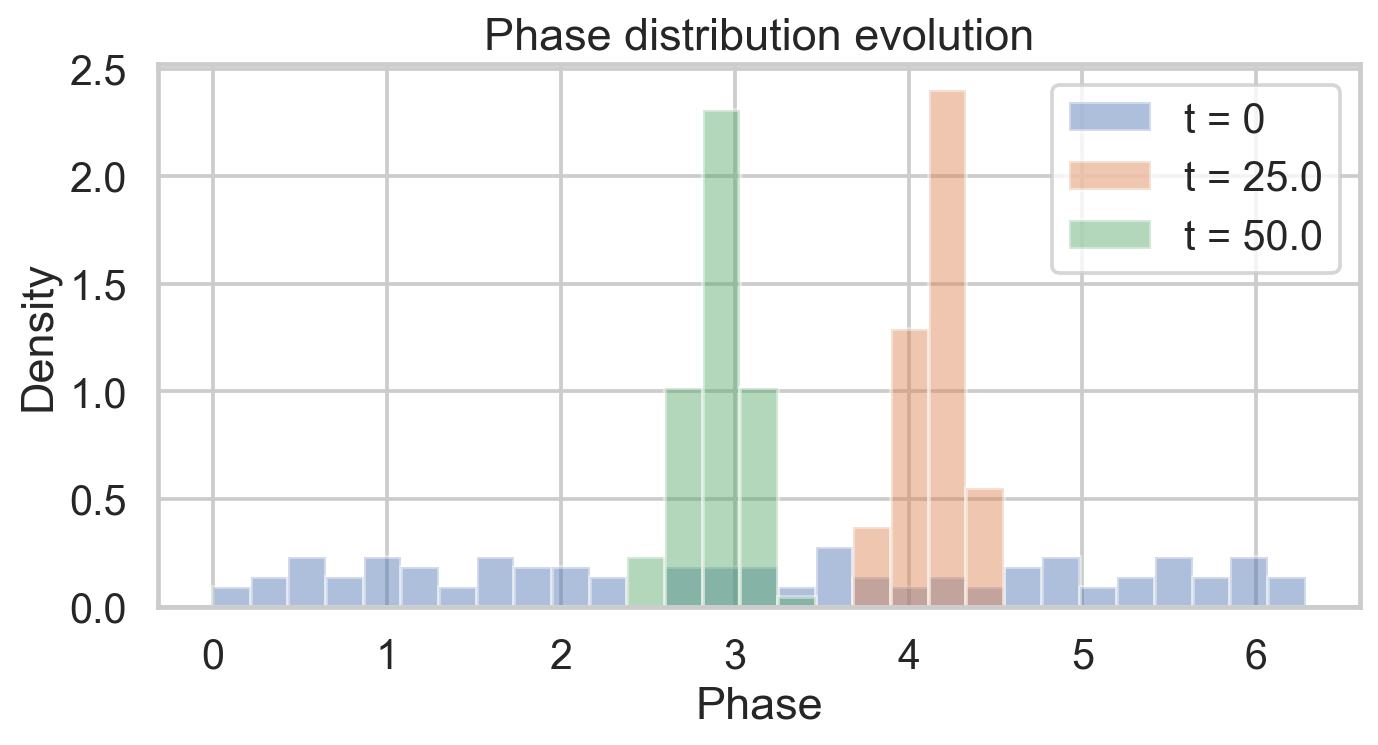
\includegraphics[width=0.8\textwidth]{phase_histograms_highK.png}
\caption{Phase distribution at different times for the synchronized run.}
\label{fig:phase_hist}
\end{figure}

At early time, phases are broad and almost uniform. At later times, the histogram becomes sharply peaked, which is a direct statistical signature of synchronization.

\subsection{Network snapshots of phase organization}

\begin{figure}[H]
\centering
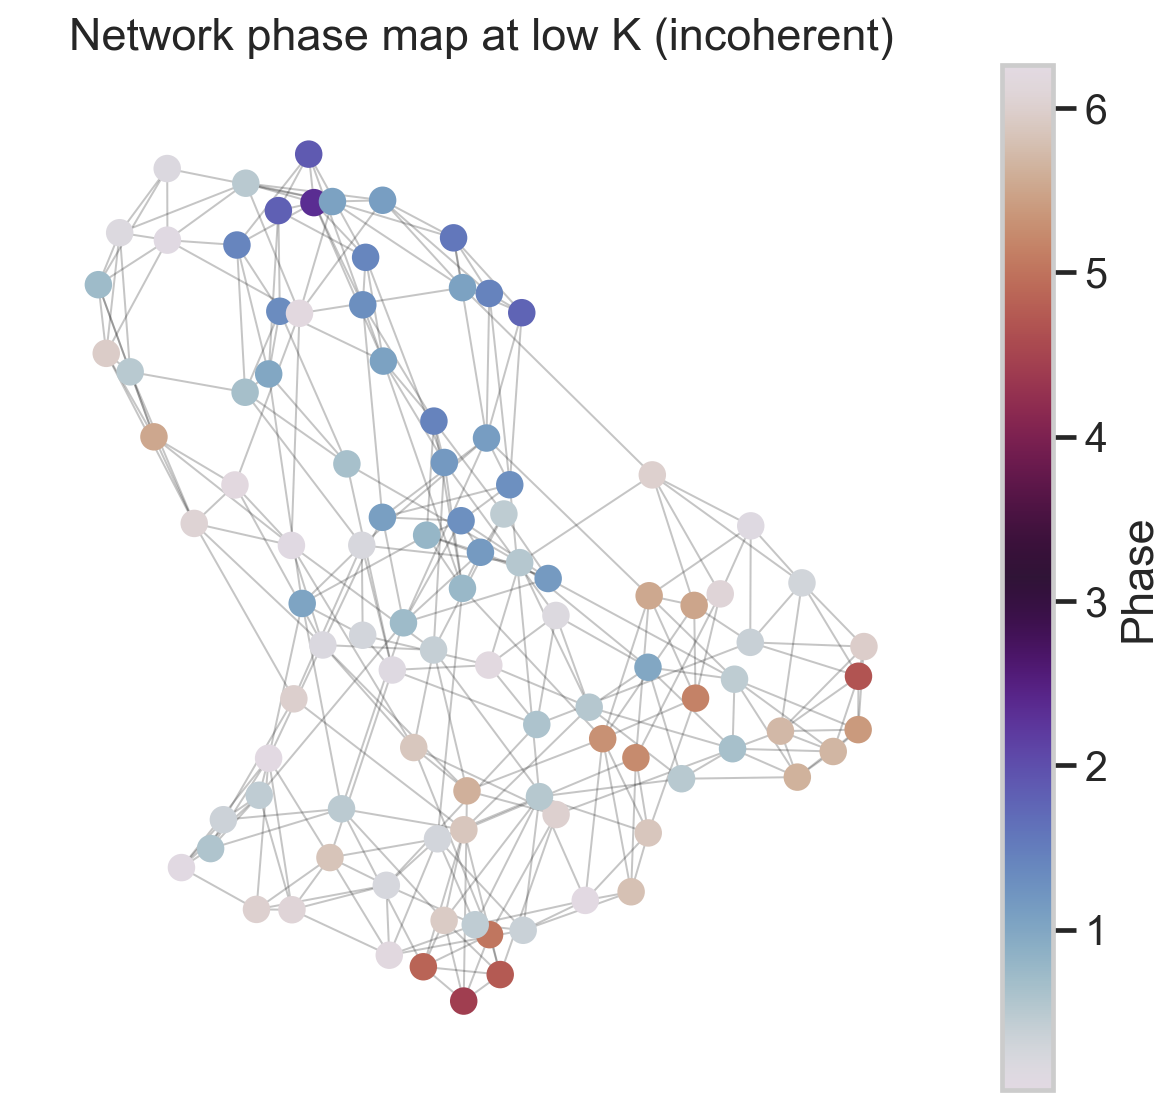
\includegraphics[width=0.8\textwidth]{network_phase_lowK.png}
\caption{Network visualization with node color as phase for low coupling.}
\label{fig:net_low}
\end{figure}

The low-coupling network has strongly mixed colors, indicating incoherent phases distributed across the graph.

\begin{figure}[H]
\centering
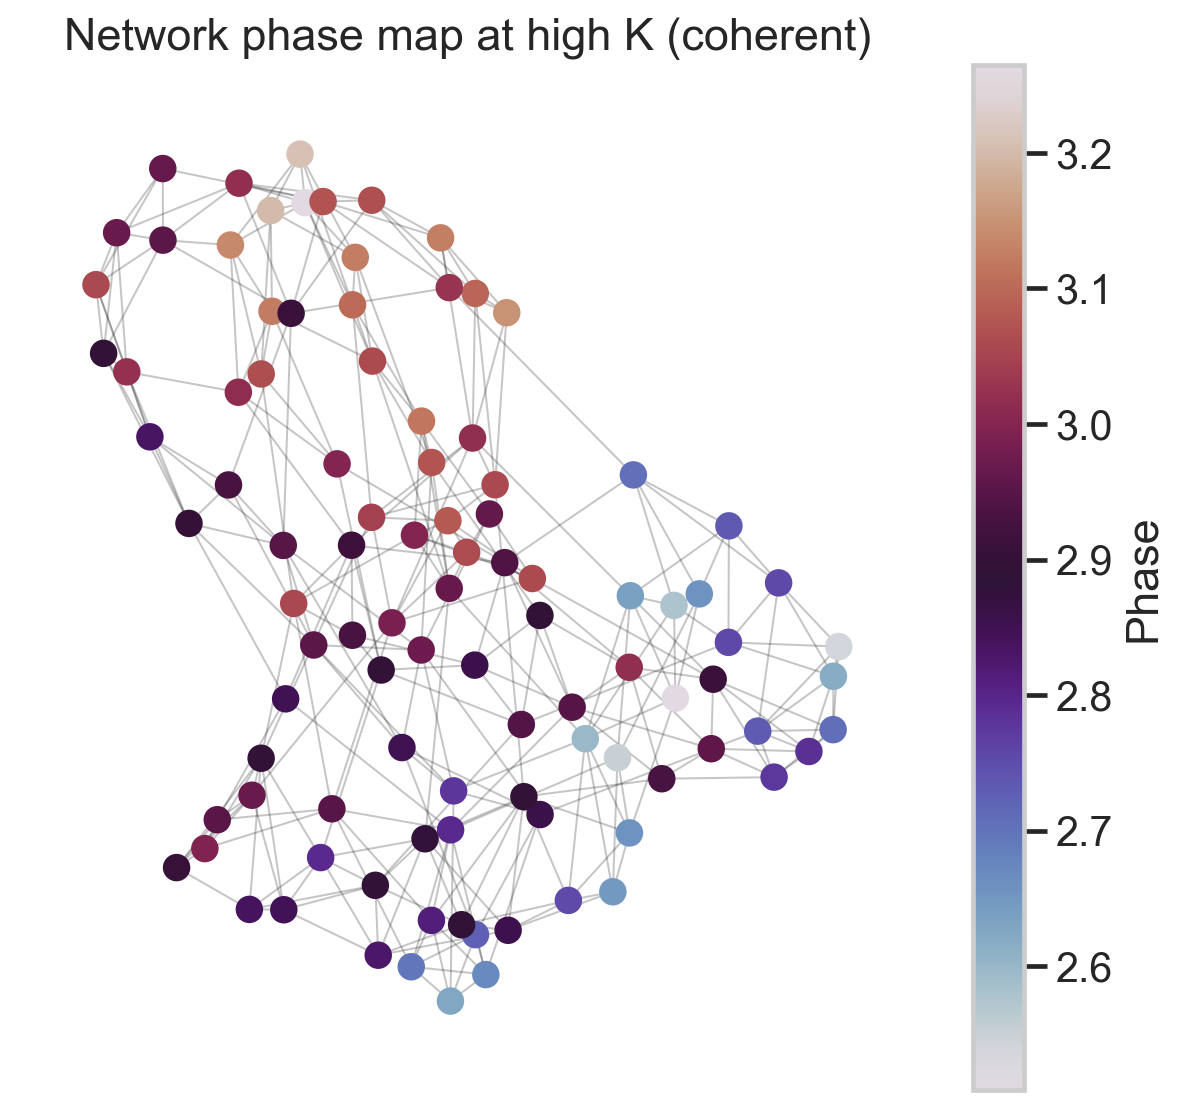
\includegraphics[width=0.8\textwidth]{network_phase_highK.png}
\caption{Network visualization with node color as phase for high coupling.}
\label{fig:net_high}
\end{figure}

At high coupling, node colors become nearly uniform. This visually confirms global phase organization on the same topology.

\subsection{Local correlation analysis}

\begin{figure}[H]
\centering
\includegraphics[width=0.8\textwidth]{correlation_matrix_highK.png}
\caption{Pairwise phase-correlation matrix $C_{ij}=\cos(\theta_i-\theta_j)$ at high coupling.}
\label{fig:corr_matrix}
\end{figure}

Most entries are close to $+1$, so many oscillator pairs are phase aligned. This is the local footprint of a synchronized network state.

\begin{figure}[H]
\centering
\includegraphics[width=0.8\textwidth]{correlation_vs_distance_highK.png}
\caption{Mean phase correlation as a function of shortest-path distance in the network.}
\label{fig:corr_distance}
\end{figure}

Correlation tends to decrease with graph distance. This behavior is physically natural because interaction influence decays through longer network paths.

\subsection{Frequency locking}

\begin{figure}[H]
\centering
\includegraphics[width=0.8\textwidth]{frequency_locking_lowK.png}
\caption{Effective frequency versus natural frequency at low coupling.}
\label{fig:lock_low}
\end{figure}

At low $K$, points are broad and remain strongly tied to natural frequency disorder. This indicates weak or absent locking.

\begin{figure}[H]
\centering
\includegraphics[width=0.8\textwidth]{frequency_locking_highK.png}
\caption{Effective frequency versus natural frequency at high coupling.}
\label{fig:lock_high}
\end{figure}

At high $K$, effective frequencies collapse into a narrow band. This is frequency entrainment, which is one of the clearest signatures of synchronization.

\subsection{Power spectrum}

\begin{figure}[H]
\centering
\includegraphics[width=0.8\textwidth]{psd_comparison.png}
\caption{Power spectral density in incoherent and synchronized regimes.}
\label{fig:psd}
\end{figure}

The incoherent regime has broader spectral content due to competing individual frequencies. In the synchronized regime, spectral power is concentrated, reflecting collective motion with reduced frequency spread.

\subsection{Effect of coupling and phase transition}

\begin{figure}[H]
\centering
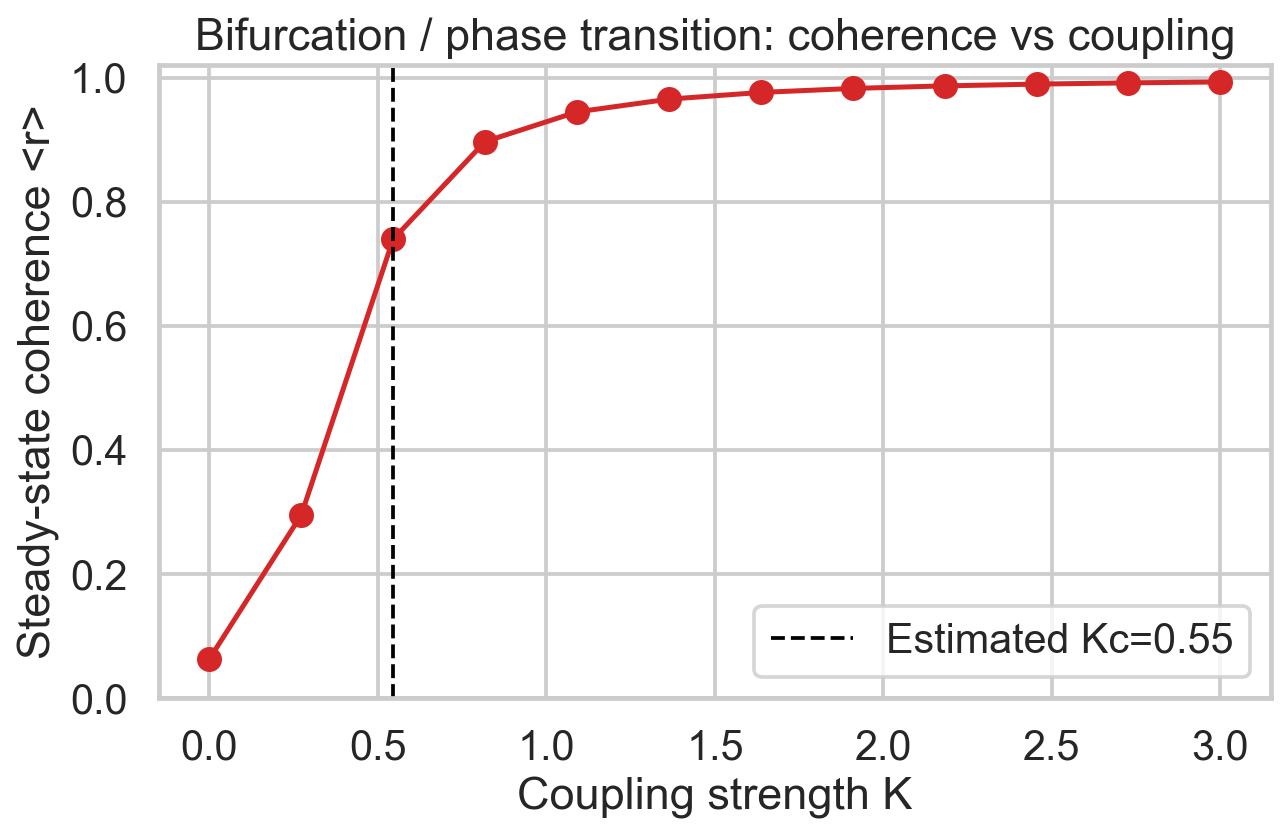
\includegraphics[width=0.8\textwidth]{bifurcation_r_vs_K_smallworld.png}
\caption{Steady-state order parameter versus coupling strength for the small-world network.}
\label{fig:rk_bifurcation}
\end{figure}

Figure \ref{fig:rk_bifurcation} shows a clear transition from low coherence to high coherence as $K$ increases. Using the implemented criterion, the estimated onset is near $K_c \approx 0.55$.

\begin{figure}[H]
\centering
\includegraphics[width=0.8\textwidth]{bifurcation_frequency_vs_K_smallworld.png}
\caption{Bifurcation-style diagram of asymptotic effective frequencies versus coupling.}
\label{fig:freq_bifurcation}
\end{figure}

The frequency branches are wide at low $K$ and collapse as $K$ increases. This shows the transition from drifting oscillators to frequency-locked collective motion.

\begin{figure}[H]
\centering
\includegraphics[width=0.8\textwidth]{sync_time_vs_K_smallworld.png}
\caption{Time to reach the synchronization threshold $r>0.9$ as a function of coupling strength.}
\label{fig:sync_time_k}
\end{figure}

Synchronization time decreases with $K$ after threshold crossing. Physically, stronger coupling gives a larger restoring pull toward phase alignment.

%-----------------------------------
\section{Bifurcation and Topology Effects}

\begin{figure}[H]
\centering
\includegraphics[width=0.8\textwidth]{topology_comparison.png}
\caption{Comparison of final coherence and synchronization speed for regular, small-world, and random networks.}
\label{fig:topology_compare}
\end{figure}

Topology strongly changes synchronization performance. In the tested window, the regular lattice synchronizes much more slowly and may not cross the strict threshold, while small-world and random networks synchronize faster and reach higher final coherence.

\begin{figure}[H]
\centering
\includegraphics[width=0.8\textwidth]{rewiring_effect_sync_time.png}
\caption{Synchronization time versus rewiring probability $p$ at fixed coupling.}
\label{fig:rewiring_effect}
\end{figure}

Even a small increase in $p$ can sharply reduce synchronization time. A few long-range shortcuts reduce characteristic path lengths, allowing phase information to spread more rapidly.

\begin{figure}[H]
\centering
\includegraphics[width=0.8\textwidth]{finite_size_effects.png}
\caption{Finite-size dependence of final coherence and synchronization time.}
\label{fig:finite_size}
\end{figure}

Finite-size behavior is visible in both observables. This is expected because fluctuations and averaging effects depend on the number of oscillators.

%-----------------------------------
\section{Discussion}

The simulations consistently show that coupling strength and topology act together to determine synchronization.

For coupling, the transition is clear. Small $K$ gives incoherent drifting phases. Larger $K$ drives phase and frequency locking, visible in $r(t)$, histograms, frequency plots, and spectra.

For topology, the regular ring is the slowest because information travels through long local paths. Rewiring introduces shortcuts, and the small-world regime improves synchronization speed while still keeping some local clustering structure. The random case tends to synchronize fastest in this parameter range.

This confirms the key small-world advantage discussed in class: short effective path lengths improve global coordination without needing all-to-all coupling.

%-----------------------------------
\section{Conclusion}

This study simulated coupled phase oscillators on Watts-Strogatz networks and focused on synchronization diagnostics.

The main conclusions are:

\begin{itemize}
	\item Synchronization emerges beyond a coupling threshold, with an estimated onset near $K_c\approx 0.55$ for the tested small-world setting.
	\item Small-world and random topologies synchronize much faster than a regular lattice in the same coupling window.
	\item A small amount of rewiring can significantly reduce synchronization time.
\end{itemize}

Overall, the results match the expected physics of network-coupled Kuramoto dynamics and give a clear quantitative picture of how structure controls collective behavior.

\end{document}
